
%%%%%%%%%%%%%%%%%%%%%%%%%%%%%%%%%%%%%%%%%%%%%%%%%%%%%%%%%%%%%%%%%%%%%%%%
%
%		Chapter 1 - Mathematical Modelling
%
%%%%%%%%%%%%%%%%%%%%%%%%%%%%%%%%%%%%%%%%%%%%%%%%%%%%%%%%%%%%%%%%%%%%%%%%


\begin{topic}[Mathematical Modelling]
%\Title{Mathematical Modelling}


In this section, we study some strategies to model problems mathematically in an effective manner.

We also provide a structure to modelling problems by breaking them in small parts:

\begin{enumerate}[label={\bf \Alph*.}]
	\item \hyperref[define]{Define the problem}
	\item \hyperref[mindmap]{Build a mind map}
	\item \hyperref[assumptions]{Make assumptions}
%	\item \hyperref[D-parvsvar]{Decide on your parameters and variables}
	\item \hyperref[model]{Construct a model}
	\item \hyperref[analysis]{Analysis of the model}
\end{enumerate}



\end{topic}


\begin{module}
	\Title{Defining Problem Statement}

	\Heading{Objectives}
	\begin{itemize}
		\item The first step in Mathematical modelling is to define the problem
		\item A good way to do this is to figure out what is the ``mathematical object'' we are looking for at the end of the process

		\item The second step is to create a mind map of the problem. This is a structured way to brainstorm possible solutions and their requirements.
	\end{itemize}
	
	\Heading{Motivation} 

\begin{annotation}
	\begin{goals}
	\Goal{Extra Reading}
	Math Modelling: Getting started and getting solutions, Bliss-Fowler-Galluzzo
	
	\hfill \qrcode{https://m3challenge.siam.org/resources/modeling-handbook}	
	\end{goals}
\end{annotation}
	\Heading{Extra Reading} \href{https://m3challenge.siam.org/resources/modeling-handbook}{Math Modelling: Getting started and getting solutions, Bliss-Fowler-Galluzzo}

\end{module}




\section*{Step A. Defining the problem}\label{define}
\addcontentsline{toc}{subsection}{Step A. Defining the problem}

The first step is to define the problem we want to solve or improve.

To do this, we should start from the end! We need to decide on what kind of mathematical object we will use in the end to show that we solved, or at least improved, the problem we were tasked with. \\


Once this is done, we can define the problem mathematically. 

\begin{example}
	Your team was tasked with optimizing the layout of an airport.
	
	You decided that in the end, to show that the team did find a good layout fo an airport, they will show
	\begin{itemize}
		\item $T = $ the total time (in minutes) necessary by the average person to walk from their airport transportation (taxi, train, bus) to their gate.
	\end{itemize}
	
	Once this decision is made, the problem to solve (or improve) becomes the following:
	
	\begin{itemize}
		\item Minimize $T$
	\end{itemize}

	There will probably be some constraints, which will be studied in Step C.

\end{example}


\vfill


\section*{Task 1.A: Elevator problem at theBigCompany}
\addcontentsline{toc}{subsection}{Task 1.A: Elevator problem at theBigCompany}


\begin{annotation}
	\begin{goals}
		\Goal{Make the question precise, bring it into a ``mathematical form''.}
		\begin{itemize}
			\item Choose a mathematical object best suited for the problem, e.g. a number, a geometric form, a graph, a function, an algorithm, ...

		\end{itemize}
	\end{goals}
%	\begin{notes}
%		
%		\begin{itemize}
%			\item There are many ways to solve this problem.
%				Some students
%				might start with equations. After they use their
%				equations to solve the problem, make them draw a picture
%				and come up with a graphical solution.
%
%			\item When the students start coming up with vector equations,
%				give them the vocabulary of \emph{linear
%				combinations}
%				and \emph{column vector notation}.
%		\end{itemize}
%	\end{notes}
\end{annotation}


You are hired by theBigCompany to help with their ``elevator problem''.

This is the email you received:

\begin{center}
	\color{blue}
	\begin{tabular}{?l}
	\begin{minipage}{.75\textwidth}
	-------- Forwarded Message -------- \\[10pt]
	\textcolor{black}{Date: } Mon, 16 September 2019 21:41:35 + 0000  \\
	\textcolor{black}{From: } CEO <theCEO@theBigCompany.ca> \\
	\textcolor{black}{To: } Human Resources <hr@theBigCompany.ca> \\
	\textcolor{black}{Subject: } they're still late !?\@\&! \\
	
	Hey Shophika! \\
	
	I still get complaints about staff being late, some by 15 minutes.
	
	With the staff we have, that's about one salary lost.
	
	Again the bottleneck of the elevators seems to be the problem.
	
	Can you suggest solutions? \\
	
	Thanks, the CEO
	\end{minipage}
	\end{tabular}
\end{center}


\vspace{5mm}

\begin{annotation}
	\begin{notes}
		
		\begin{itemize}
			\item Students will start discussing how to solve the problem
			\item This question deals with what will happen \textbf{after} solving the problem
			\item The goal of this question is to think about how to best tell a ``mathematically-challenged'' CEO that you solved the problem
		\end{itemize}
	\end{notes}
\end{annotation}

\paragraph{Scenario 1:}

With your team, you must decide on one answer and be prepared to report on your decision and the reason for your choice.

\subparagraph{Task.} What mathematical object would you use to convince the CEO that you have solved or improved the problem?








\newpage



\question
\label{object}
For each part, what ``mathematical object'' would you use to communicate that you have solved or improved the problem? Then define the problem mathematically.
\begin{parts}
	\item Help the city of Toronto choose the best recycling centre.
	\item Help the Canadian Institute of Health Information (CIHI) estimate how significant the outbreak of illnesses will be in the coming year in Canada.
	\item Create a mathematical model to rank roller coasters according to thrill factor.
	\item Gas stations offer different prices for gas. I would like to create an app that finds the best gas station to go to. What should ``best'' mean?
	\item The mayor of Toronto wants to extend the subway line with a new \textcolor{RoyalBlue}{blue line} as in Figure \ref{TTC}. Is it optimal?
	
	\item Is it better to buy or rent? 
	\begin{enumerate}
		\item Is it better to buy a car or rent Zipcar, Enterprise Carshare, or Car2go?
		\item Does the criteria you used to evaluate the previous question change if the question is whether to buy a bicycle or use Bike Share Toronto? 
	\end{enumerate}

	\begin{center}
	\begin{figure}[!htbp]
	\includegraphics*[width=500pt]{images/TTC-extension.png}
	\caption{Extension plans for Toronto subway line.}
	\label{TTC}	
	\end{figure}
	\end{center}
	
\end{parts}








\newpage

\section*{Step B. Building a mind map}\label{mindmap}
\addcontentsline{toc}{subsection}{Step B. Building a mind map}

A mind map is a tool to visually outline and organize ideas. Typically a key idea is the centre of a mind map and associated ideas are added to create a diagram that shows the flow of ideas. In Figure \ref{mindmap1}, we focus on the definition of ``best'', with three possible definitions
branching off to be further explored. From here, we can focus our attention on one of the three branches
at a time.

\begin{figure}[!htbp]
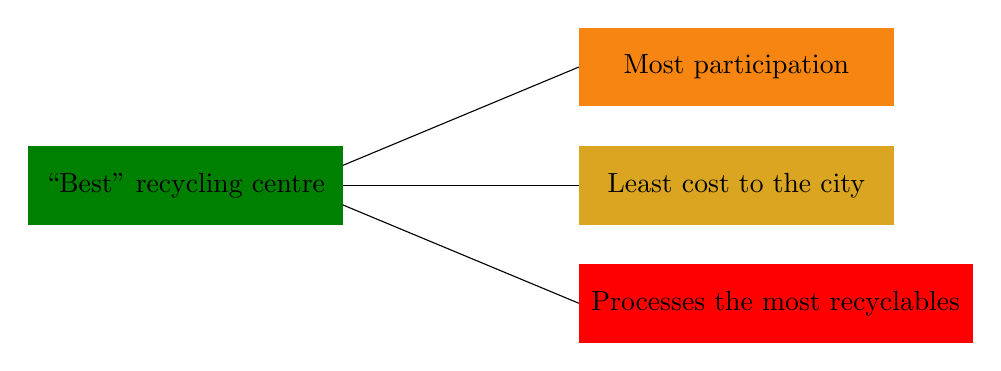
\begin{tikzpicture}
	\fill[color=Green] (0,0) rectangle (4,1) node[pos=.5] {\color{black}``Best'' recycling centre};
	\fill[color=BurntOrange] (7,2.5) rectangle (11,1.5) node[pos=.5] {\color{black}Most participation};
	\fill[color=Goldenrod] (7,0) rectangle (11,1) node[pos=.5] {\color{black}Least cost to the city};
	\fill[color=red] (7,-1.5) rectangle (12,-0.5) node[pos=.5] {\color{black}Processes the most recyclables};
	\draw (4,0.75) -- (7,2);
	\draw (4,0.5) -- (7,0.5);
	\draw (4,0.25) -- (7,-1);
\end{tikzpicture}
\caption{An example of a simple mind map.}
\label{mindmap1}
\end{figure}


Let's think about the least-cost option first. We probably can't determine how much any recycling program costs without knowing more about the recycling program, so a good place to start is to ask the question ``What kinds of recycling programs exist?''
If we aren't familiar with different types of recycling, we might need to do some research to see what kinds of programs exist.


A possible next step on your mind map for the least-cost approach could be the one shown in Figure \ref{mindmap2}.

\begin{figure}[!htbp]
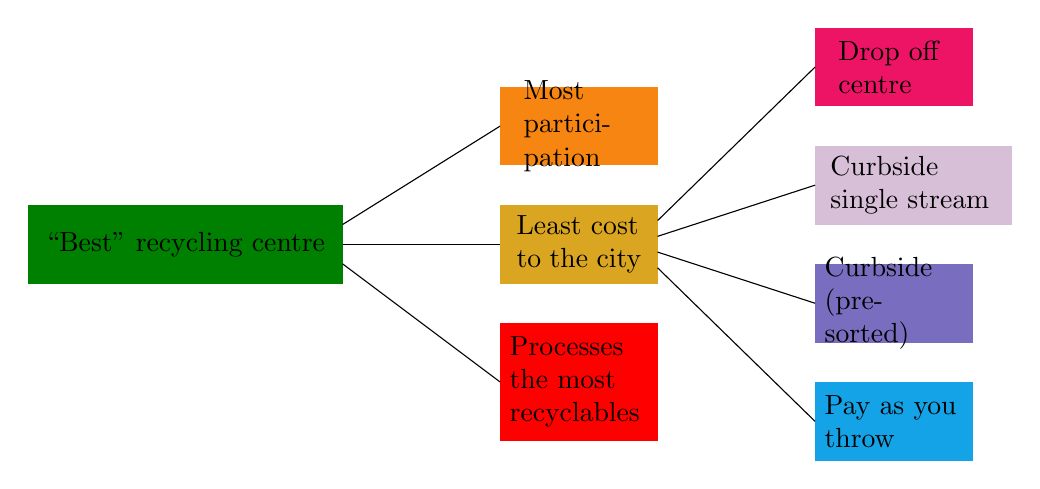
\begin{tikzpicture}
	\fill[color=Green] (0,0) rectangle (4,1) node[pos=.5] {\color{black}``Best'' recycling centre};
	\fill[color=BurntOrange] (6,2.5) rectangle (8,1.5) node[pos=.5] {\color{black}\begin{minipage}{40pt}\raggedright Most participation\end{minipage}};
	\fill[color=Goldenrod] (6,0) rectangle (8,1) node[pos=.5] {\color{black}\begin{minipage}{45pt}\raggedright Least cost to the city\end{minipage}};
	\fill[color=red] (6,-2) rectangle (8,-0.5) node[pos=.5] {\color{black}\begin{minipage}{50pt}\raggedright Processes the most recyclables\end{minipage}};
	\draw (4,0.75) -- (6,2);
	\draw (4,0.5) -- (6,0.5);
	\draw (4,0.25) -- (6,-1.25);
	\fill[color=WildStrawberry] (10,2.25) rectangle (12,3.25) node[pos=.5] {\color{black}\begin{minipage}{40pt}\raggedright Drop off centre\end{minipage}};	
	\fill[color=Thistle] (10,0.75) rectangle (12.5,1.75) node[pos=.5] {\color{black}\begin{minipage}{60pt}\raggedright Curbside single stream\end{minipage}};	
	\fill[color=Periwinkle] (10,0.25) rectangle (12,-0.75) node[pos=.5] {\color{black}\begin{minipage}{50pt}\raggedright Curbside (pre-sorted)\end{minipage}};	
	\fill[color=Cerulean] (10,-2.25) rectangle (12,-1.25) node[pos=.5] {\color{black}\begin{minipage}{50pt}\raggedright Pay as you throw\end{minipage}};
	\draw (8,0.8) -- (10,2.75);	
	\draw (8,0.6) -- (10,1.25);	
	\draw (8,0.4) -- (10,-0.25);	
	\draw (8,0.2) -- (10,-1.75);	
\end{tikzpicture}
\caption{Next step of a mind map.}
\label{mindmap2}
\end{figure}



\begin{annotation}
	\begin{goals}
		\Goal{Software}

		There is free online software to help creating a mind map. One such is \href{http://freemind.sourceforge.net}{FreeMind}.
		
		\hfill \qrcode{http://freemind.sourceforge.net}	
	\end{goals}
\end{annotation}

%
%\subparagraph{Software.} There is free online software to help creating a mind map. One such is \textcolor{blue}{\underline{\href{http://freemind.sourceforge.net}{FreeMind}}}.






\newpage

\begin{annotation}
	\begin{notes}
	\begin{itemize}
		\item Students usually come up with more complicated variations:
		\begin{itemize}
			\item Money spent on late employees' salaries
			\item sum of time in minutes that employees are late counting only employees that are at most 15 minutes late
		\end{itemize}
		\item Stick with $R$, a simple first approach
	\end{itemize}	
	\end{notes}
	
\end{annotation}

\section*{Task 1.B: Elevator problem at theBigCompany}
\addcontentsline{toc}{subsection}{Task 1.B: Elevator problem at theBigCompany}


\paragraph{Scenario 2:} \label{elevatorR}

Your team decides that the mathematical object you will use to show the CEO that you solved or improved the problem is
\begin{itemize}
	\item $R=$ the sum in minutes by which every employee is late.
\end{itemize}

Employees that are on time count for 0 minutes. 

\subparagraph{Task.} Create a mind map for the question: \quad How can $R$ be minimized?


\vfill

\question

For each part, create a mind map. Focus on the same approach you had for question \ref{object}.
\begin{parts}
	\item Help the city of Toronto choose the best recycling centre.
	\item Help the Canadian Institute of Health Information (CIHI) estimate how significant the outbreak of illnesses will be in the coming year in Canada.
	\item Create a mathematical model to rank roller coasters according to thrill factor.
	\item Gas stations offer different prices for gas. I would like to create an app that finds the best gas station to go to. What should ``best'' mean?
	\item The mayor of Toronto wants to extend the subway line with a new blue line as in Figure \ref{TTC}. Is it optimal?
	
	\item Is it better to buy a car or rent Zipcar, Enterprise Carshare, or Car2go?

	
\end{parts}








\begin{module}
	\Title{Making Assumptions}
	
	\Heading{Objectives}
	\begin{itemize}
		\item Bla bla bla	
	\end{itemize}
	
	\Heading{Motivation} 


\begin{annotation}
	\begin{goals}
	\Goal{Extra Reading}
	Math Modelling: Getting started and getting solutions, Bliss-Fowler-Galluzzo
	
	\hfill \qrcode{https://m3challenge.siam.org/resources/modeling-handbook}	
	\end{goals}
\end{annotation}
	\Heading{Extra Reading} \href{https://m3challenge.siam.org/resources/modeling-handbook}{Math Modelling: Getting started and getting solutions, Bliss-Fowler-Galluzzo}


\end{module}







\section*{Step C. Making Assumptions}\label{assumption}
\addcontentsline{toc}{subsection}{Step C. Making Assumptions}






Real problems are complex, so when modelling a real problem mathematically, we must make some assumptions. 

The assumptions that we make will affect the problem we are solving and its difficulty, so we need to strike a balance between:
\begin{itemize}
\item accuracy -- the fewer assumption the better, and
\item solvability -- the more assumptions the better.
\end{itemize}

\begin{annotation}
	\begin{goals}
		When building a mind map, keep track of the assumptions necessary for each step.
	\end{goals}
\end{annotation}

Many assumptions follow naturally when building a mind map. \\


\begin{annotation}
	\begin{goals}
		Remember to justify all your assumptions.
	\end{goals}
\end{annotation}
When figuring which assumption to make, keep in mind the key-factors of the problem and find data when available (usually online), if not available, measure data when possible, and if it's not possible, make a reasonable assumption on what the data might look like.

Another thing to keep in mind are \emph{time constraints}. Whether in a class, test, or working in a project, there will be deadlines. Your assumptions should take time constraints into consideration. 

\hfill \\

%	\section*{Step D. Parameters or Variables?}\label{D-parvsvar}
%	\addcontentsline{toc}{subsection}{Step D. Parameters or Variables?}
%	
%	
%	
%	When you have defined the problem you want to solve and you have made your (initial) assumptions, it is then time to define some details of the problem.
%	
%	
%	
%	
%	With the problem statement clearly defined and an initial set of assumptions made (a list that will likely get longer), you are ready to start to define the details of your model. Now is the time to pause to ask what
%	is important that you can measure. Identifying these notions as variables, with units and some sense of their range, is key to building the model.
%	The purpose of a model is to predict or quantify something of interest. We refer to these predictions
%	as the outputs of the model. Another term we use
%	for outputs is dependent variables. We will also have independent variables, or inputs to the model. Some quantities in a model might be held constant, in which case they are referred to as model parameters. Let's look at a few simple examples that will help you distinguish between these concepts. We'll also see how they depend on your viewpoint and the problem statement.
%	
%	
%	
%	%There is a clear difference between \emph{variables} and \emph{parameters}. 
%	
%	\begin{definition}[Variables and Parameters]
%	
%	
%	A \emph{variable} represents a model state, and may change during simulation.
%	
%	A \emph{parameter} is commonly used to describe objects statically. A \emph{parameter} is normally a constant in a single simulation, and is changed only when you need to adjust your model behaviour. 
%	\end{definition}
%	
%	%Use a variable instead of a parameter if you need to model some data unit continuously changing over time. Use a parameter instead of a variable if you just need to model some parameter of an object changed only at particular moments of time.
%	
%	
%	
%	\begin{annotation}
%		\begin{goals}
%		\qrcode{https://en.wikipedia.org/wiki/Parameter\#Mathematical\_models}	
%		\end{goals}
%	\end{annotation}
%	\begin{note}{(from Wikipedia)}
%	The quantities appearing in the equations we classify into variables and parameters. The distinction between these is not always clear cut, and it frequently depends on the context in which the variables appear. 
%	
%	Usually a model is designed to explain the relationships that exist among quantities which can be measured independently in an experiment; these are the \emph{variables} of the model. 
%	
%	To formulate these relationships, however, one frequently introduces ``constants'' which stand for inherent properties of nature (or of the materials and equipment used in a given experiment). These are the \emph{parameters}.	
%	\end{note}






%
%
%
%The choice of question in the previous module should determine the \emph{dependent} variable.

%
%The \emph{parameters} are the independent variables in the problem, e.g. the speed of the elevators. The final answer will depend on the parameters in the problem. 
%
%We can estimate the parameters, and sometimes even change them. \\
%
%The \emph{variables} are dependent. This meant that if we change the parameters, the variables will change automatically. 




\vfill





\section*{Task 1.C: Elevator problem at theBigCompany}
\addcontentsline{toc}{subsection}{Task 1.C: Elevator problem at theBigCompany}


We now give you some technical details about theBigCompany:


\begin{itemize}
	\item The company occupies the floors 30--33 of the building Place Ville-Marie (in Montr\'eal).

	\item Personnel is distributed in the following way: 
	\begin{itemize}
		\item 350 employees in floor 30,
		\item 350 employees in floor 31,
		\item 250 employees in floor 32, 
		\item 150 employees in floor 33.
	\end{itemize}
\end{itemize}

\textsl{Note.} Even though these details are fictional, the numbers respect the building code.


\subparagraph{Tasks.} Focus on a \textbf{few} parameters and variables. State hypotheses.

\begin{annotation}
	\begin{notes}
		\begin{itemize}
			\item Students usually have trouble starting. 
			\item They usually agree that they have to figure out how elevators work, so you can prompt them to be more specific. 
			
			\item In the end they should come up with questions like these:
			\begin{itemize}
				\item How fast are the elevators?
				\item How much time do elevators take in each floor?
				\item How many floors do elevators stop on their way up?
				\item How many people fit in the elevator?
				\item Should we consider elevator failures?
			\end{itemize}
		\end{itemize}	
	\end{notes}
\end{annotation}

\begin{enumerate} 

	\item With your team, decide on what kind of information you would need to have to be able to solve this problem.

	\item Find the relevant information about the elevators (search the internet, by experimentation). Check the reliability of the data you found.

	\item For the relevant information that you cannot obtain, make assumptions. These assumptions should be reasonable and you should be able to justify them.
\end{enumerate}

%\vspace{0.5in}

\newpage
%\vfill



\question
For each part, you are required to make an estimate for some quantity. Make assumptions and justify them in order to solve the problem.
\begin{parts}
	\item What is the number of piano players in Toronto? \hfill \emph{(Fermi problem)}
	\item How many linear km of roads are there in Toronto?
	\item How much salt the city of Toronto needs for its roads during the Winter?
	\item The skating season in Canada is shortening: What are the key-factors determining its length?
	
\end{parts}












\begin{module}
	\Title{Building Solutions}
	
	\Heading{Objectives}
	\begin{itemize}
		\item Bla bla bla	
	\end{itemize}
	
	\Heading{Motivation} 

\begin{annotation}
	\begin{goals}
	\Goal{Extra Reading}
	Math Modelling: Getting started and getting solutions, Bliss-Fowler-Galluzzo
	
	\hfill \qrcode{https://m3challenge.siam.org/resources/modeling-handbook}	
	\end{goals}
\end{annotation}
	\Heading{Extra Reading} \href{https://m3challenge.siam.org/resources/modeling-handbook}{Math Modelling: Getting started and getting solutions, Bliss-Fowler-Galluzzo}
\end{module}









\section*{Step D. Construction of a Model}\label{model}
\addcontentsline{toc}{subsection}{Step D. Construction of a Model}


This is the part of the modelling where we connect all that we have done so far: the problem we defined, the mind map, the assumptions, and all the variables and parameters in a mathematical model to answer the ``mathematical'' problem defined in \hyperref[define]{Step A}.

This usually means writing down mathematical equations, constructing a graph, analyzing a geometric figure, or do some statistical analysis. \\


\begin{example}
Your team is tasked with finding the best recycling centre (we looked at this example in \hyperref[mindmap]{Step B}) and your  team has chosen to minimize the cost to the city by using drop off centres.

As part of modelling process, your team has made the following assumptions/measurements:
\begin{itemize}
	\item People would be willing to pay \$2.29 to recycle per month or \$0.53 per week
	\item People would make bi-weekly trips to the centre
	\item Gasoline costs around \$1.26 per litre
	\item On average a passenger car needs 10 litres per hundred kilometres
\end{itemize}

This means that the (one-way) distance people are willing to travel every week to the drop-off centre is
$$
d \;=\; \frac{1}{4.3 \text{ trips/month}} \cdot \frac{\$2.29 / {\text{month}} }{(\$1.26 \text{/L}) \ \cdot\  (0.1 \text{ L / km})} \;=\; 4.2 \text{  km/trip}.
$$

This should help us figure out the best way to place the drop-off centres:

The Mathematical model might look like this

\begin{itemize}
	\item Maximize (number of people within a 4.2 km radius of a drop-off centre)
	\item subject to a certain number of drop-off centres (given by the city budget)
\end{itemize}

	
\end{example}

\hfill

Sometimes, the mathematical tools necessary to tackle the problem are clear, but often they are not. In those cases it may be helpful to analyze some simple cases.









\vfill



\section*{Task 1.D: Elevator problem at theBigCompany}
\addcontentsline{toc}{subsection}{Task 1.D: Elevator problem at theBigCompany}


With the same details as before in \hyperref[assumptions]{step C}, write down a mathematical model for this problem.


\newpage

\question
For each part, create a model to answer the question. Remember all the previous steps.

\begin{parts}\label{models1}
	\item You want to open a piano store in Toronto, where should you open it?
	\item There was a big snow storm in Toronto and the roads need cleaning. How should the city deploy its snow plowers?
	\item The city of Toronto wants to deactivate the Pickering nuclear power plant in favour of renewable power sources. What is the best way to create the same amount of electricity using only renewable sources in the GTA?
	\item Loblaws wants to start an online food delivery service. How should they do it?
	\item The city airport (YTZ) built a tunnel to access the island airport from the city. Before that, they used a ferry. Was building the tunnel a good decision?	
\end{parts}







\begin{module}
	\Title{Model Assessment}
	
	\Heading{Objectives}
	\begin{itemize}
		\item Bla bla bla	
	\end{itemize}
	
	\Heading{Motivation} 

\begin{annotation}
	\begin{goals}
	\Goal{Extra Reading}
	Math Modelling: Getting started and getting solutions, Bliss-Fowler-Galluzzo
	
	\hfill \qrcode{https://m3challenge.siam.org/resources/modeling-handbook}	
	\end{goals}
\end{annotation}
	\Heading{Extra Reading} \href{https://m3challenge.siam.org/resources/modeling-handbook}{Math Modelling: Getting started and getting solutions, Bliss-Fowler-Galluzzo}

\end{module}




\section*{Step E. Analysis of the Model}\label{analysis}
\addcontentsline{toc}{subsection}{Step E. Analysis of the Model}


At this point, you have defined a problem statement, and a mind map to help you decide how to approach the problem. You have made assumptions and made note of them and justified them.
You finally created a model to solve the problem.

The next step is to analyze the model.

There are two types of analysis:


\paragraph{\textcolor{cyan}{\textbf{Superficial assessment.}}} Are the units correct? Are the variables and parameters of a reasonable magnitude? Does it behave as expected? Does it make sense?



\paragraph{\textcolor{cyan}{\textbf{In-depth assessment.}}} Once the superficial assessment is verified, we need to understand the model at a deeper level. 

What are the model's strengths? What are its weaknesses?

When you change the inputs of the model, how do the outputs change? This is called {\emph sensitivity analysis}. 


Next is a simple example adapted from \cite{bliss}.


\begin{annotation}
	\begin{goals}
	\Goal{Desmos Graph}
	\hfill \qrcode{https://www.desmos.com/calculator/z9cftzus0z}	
	\end{goals}
\end{annotation}

\begin{example}[Modelling the flu]

History of the project:
\begin{itemize}
	\item Split population into two classes: \emph{infected} and \emph{not infected}
	\item Assume that each infected person infects $R$ number of non infected people every $b$ days
	\item Define $I(n) = $ number of infected people after $n$ days
	\item The two previous points imply \quad $I(n \cdot b) = R \cdot I(n)$
	\item We can then conclude that \quad $I(n b) = (1+R)^n \, I(0)$ \hfill (why?)
\end{itemize}

After plotting the resulting function $I(n)$ (click or follow the QR code on the right), we can assess our model:

\emph{Strengths:}
\begin{itemize}
	\item After two days $(b=2)$, there are 6 infected people, so it is following our assumption
	\item The number of infected people increases faster and faster as expected 
	\item The disease spreads at a constant rate. Also on Desmos, check the infection rate $\dfrac{I(n+b)}{I(n)}$
	\item We could find an explicit formula for the number of infected individuals $I(n)$
\end{itemize}


\emph{Weaknesses:}
\begin{itemize}
	\item The model is too simple, so it doesn't model the spread of the flu accurately
	\item The model an exponential rate of infection, which is not possible for very long
	\item The model predicts that eventually the disease will spread to everyone
	\item The model assumes that there are only two types of people: infected and susceptible. Do people recover from the disease?
\end{itemize}

\end{example}




After assessing the model, if time allows, it is important to re-think the model and the assumptions made.





\section*{Task 1.E: Elevator problem at theBigCompany}
\addcontentsline{toc}{subsection}{Task 1.E: Elevator problem at theBigCompany}


Continuing on the elevator problem, let us think of this model for the problem.

\textbf{Facts:}
\begin{itemize}
	\item Loading time of people at ground floor = 20 s
	\item Speed of uninterrupted ascent/descent = 1.5 floors/s
	\item Stop time at a floor = 7 s
	\item Number of elevators serving floors 30--33 = 8

	(these elevators serve floors 23-33 = 11 floors)
	
	\item Maximal capacity of elevators = 25 people
\end{itemize}


\textbf{Assumptions:}
\begin{itemize}
	\item Personnel that should start at time $t$, arrive uniformly in the interval $[t-30, t-5]$ in minutes
	\item First arrived, first served
	\item During morning rush hour, elevators don't stop on the way down
	\item Elevators stop only at half the floors they serve
	\item Elevator failures are neglected
	\item Mean number of people per floor is equal to the mean number of people per floow of the BigCompany
	\item Elevators are filled, in average, to 80\% of their capacity
\end{itemize}


\textbf{Model:}
\begin{itemize}
	\item Mean number of people per floor $= d = \dfrac{350+350+250+150}{4} = 275$ people / floor
	\item Number of people on floors served by elevators (11 floors) $= N = d \cdot 11 = 3025$ people
	\item Time $\Delta t$ of one trip

\hfil $\Delta t \quad = \quad $ \framebox{$\substack{\text{loading time on}\\\text{ground floor}}$} 
		$ \;+ \;$ \framebox{$\substack{\text{time of flight}\\\text{ground $\to 33$}}$}
		$ \;+\; $ \framebox{$\substack{\text{time of flight}\\\text{$33 \to$ ground}}$}
		$\;+\; $ \framebox{$\substack{\text{stop time to}\\\text{6 of the 11 floors}}$} $\quad = \quad$ 106 s
		
		\item Number of trips necessary per elevator $= n = \dfrac{3025}{20 \cdot 8} \approx 19$ trips

		\item Time necessary to carry the staff of the BigCompany $= \pmb{t} = \dfrac{19 \cdot 106}{60} = 33 $ minutes
\end{itemize}

\hfill \\

\begin{annotation}
	\begin{notes}

Some questions to guide the students:
	\begin{itemize}
	\item What are the strengths?
	\item What are the weaknesses?
	\item Is the result around what you expected?
\end{itemize}	
	
\hfill \\
In case students don't realize that something is wrong:
\begin{itemize}
	\item People start arriving 30 minutes before the starting time, so \emph{everybody will be on time?}
	\item Assume that the CEO of the BigCompany is right: people are arriving late! What's wrong with the model?

	\item Which assumptions should be relaxed? Or checked?
	\item If one needs to be replaced, by what?
	\end{itemize}
	
	\end{notes}
\end{annotation}

Your task is to assess this model.
Be ready to report on your assessment.




\newpage

\question
Assess the models created in question \ref{models1}:

\begin{parts}
	\item You want to open a piano store in Toronto, where should you open it?
	\item There was a big snow storm in Toronto and the roads need cleaning. How should the city deploy its snow plowers?
	\item The city of Toronto wants to deactivate the Pickering nuclear power plant in favour of renewable power sources. What is the best way to create the same amount of electricity using only renewable sources in the GTA?
	\item Loblaws wants to start an online food delivery service. How should they do it?
	\item The city airport (YTZ) built a tunnel to access the island airport from the city. Before that, they used a ferry. Was building the tunnel a good decision?	
\end{parts}







\begin{module}
	\Title{Putting it all together}
	\Heading{Textbook} \href{https://m3challenge.siam.org/resources/modeling-handbook}{Math Modelling: Getting started and getting solutions, Bliss-Fowler-Galluzzo}
	
	\Heading{Objectives}
	\begin{itemize}
		\item Bla bla bla	
	\end{itemize}
	
	\Heading{Motivation} 


\end{module}




\section*{Step F. Writing a report}\label{F-report}
\addcontentsline{toc}{subsection}{Step F. Writing a report}



